\documentclass[9pt,twocolumn]{extarticle}
\usepackage[letterpaper,margin=0.68in,top=0.71in,bottom=1.05in]{geometry}
\usepackage{mathptmx}
\usepackage{graphicx}
\graphicspath{{figures/}}
\usepackage{booktabs}
\usepackage{array}
\usepackage{tikz}
\usepackage{pgfplots}
\pgfplotsset{compat=1.18}
\usepackage[hidelinks]{hyperref}
\usepackage[capitalize,nameinlink]{cleveref}
\usepackage{microtype}
\usepackage{caption}
\captionsetup{font=footnotesize}
\setlength{\columnsep}{0.22in}
\setlength{\parindent}{1em}
\setlength{\parskip}{0pt}
\title{Country Clustering of ICT Worker Issues: A Comparative Analysis of 37 Economies}
\author{%
\begin{tabular}[t]{@{}c@{\hspace{2.5em}}c@{}}
\textit{Suryansh Rohil} & \textit{Anant Atreya}\\
2310110314 & 2310110038\\
sr738@snu.edu.in & aa854@snu.edu.in\\
Greater Noida, India & Greater Noida, India\\
\end{tabular}\\[0.6em]
\textit{Instructor: Mr. Jaideep Ghosh}\\
Course: DOM207--DOM3007--DOM6401%
}
\date{}
\begin{document}
\twocolumn[\maketitle\begin{abstract}
We clustered 37 countries on two supplied scores for each of nine ICT-worker issues. K-means assignments at $k=2$ are identical for Score A, Score B, and the combined 18-feature set (ARI=1.000); Ward clustering returns the same split. The combined solution has 17 countries in one group and 20 in the other. Its mean silhouette is 0.321. Average linkage produces a different partition. The score construction and direction are undocumented, so these groups describe score profiles; they do not rank national ICT labor markets.
\end{abstract}\vspace{1.0em}]

\section{Introduction}
The IMF asked whether 37 countries can be grouped by ICT workers' responses across nine issues. We compare the two recorded scores per issue, test how assignments change with feature set and clustering method, and read the resulting profiles against macroeconomic context. The issues are friendship-circle support (FC), job insecurity (JI), self-efficacy (SE), work satisfaction (WS), work overload (WO), work--home conflict (WH), work exhaustion (WE), turnover intention (TI), and intention to leave the ICT profession (TA)~\cite{task,definitions}.

At $k=2$, k-means and Ward agree across all three feature sets. Average linkage does not. The split describes these observations; no income, labor-market, education, infrastructure, or policy covariates were supplied to explain it.

\section{Data Preprocessing}
The workbook has 37 country rows and 21 columns: country, code, sample size (\texttt{Num}), and 18 issue scores. We matched each score pair to the nine issue codes in the definitions PDF. No values are missing. We retained all countries and features; no values were imputed or removed. Sample size ranges from 93 to 634 (median 300) and was excluded from the distance matrix.

We standardized each feature to zero mean and unit variance before calculating Euclidean distances. Score A and Score B each contribute nine dimensions; the combined model contributes all 18. Standardization prevents raw units from setting the distances. Correlated scores can still give related issues extra weight.

Within-issue score correlations range from $r=0.927$ to $0.998$. The largest off-diagonal issue correlation is 0.837 for Score A and 0.863 for Score B. PCA on the combined standardized matrix assigns 51.6\% of variance to PC1 and 72.0\% to the first two components; three components account for 80.7\%. We retained the original dimensions for clustering and profiling.

Three standardized values exceed $|z|=3$: Iran on Score A self-efficacy, Iran on Score B self-efficacy, and Nigeria on Score B work--home conflict. We retained them. Removing each country in turn leaves the two-group partition unchanged (minimum ARI=1.000); this checks single-country influence, not alternative scaling. The PDFs do not document score direction or construction; correlation between the score pairs does not resolve either point.

\section{Data Visualization}
For each feature set, the largest mean silhouette among $k=2$--6 occurs at $k=2$ (\Cref{fig:silhouette}). The combined score falls from 0.321 at $k=2$ to 0.299 at $k=3$. This margin is small. A silhouette measures separation in the chosen distance space, not economic validity.

\Cref{fig:dend_a,fig:dend_b,fig:dend_both} show the Ward merges for Score A, Score B, and all 18 features. The dashed line marks the $k=2$ cut. Country labels permit inspection of nearby cases and large merges; the tree alone cannot establish an economic grouping.

\begin{figure*}[!t]
\centering
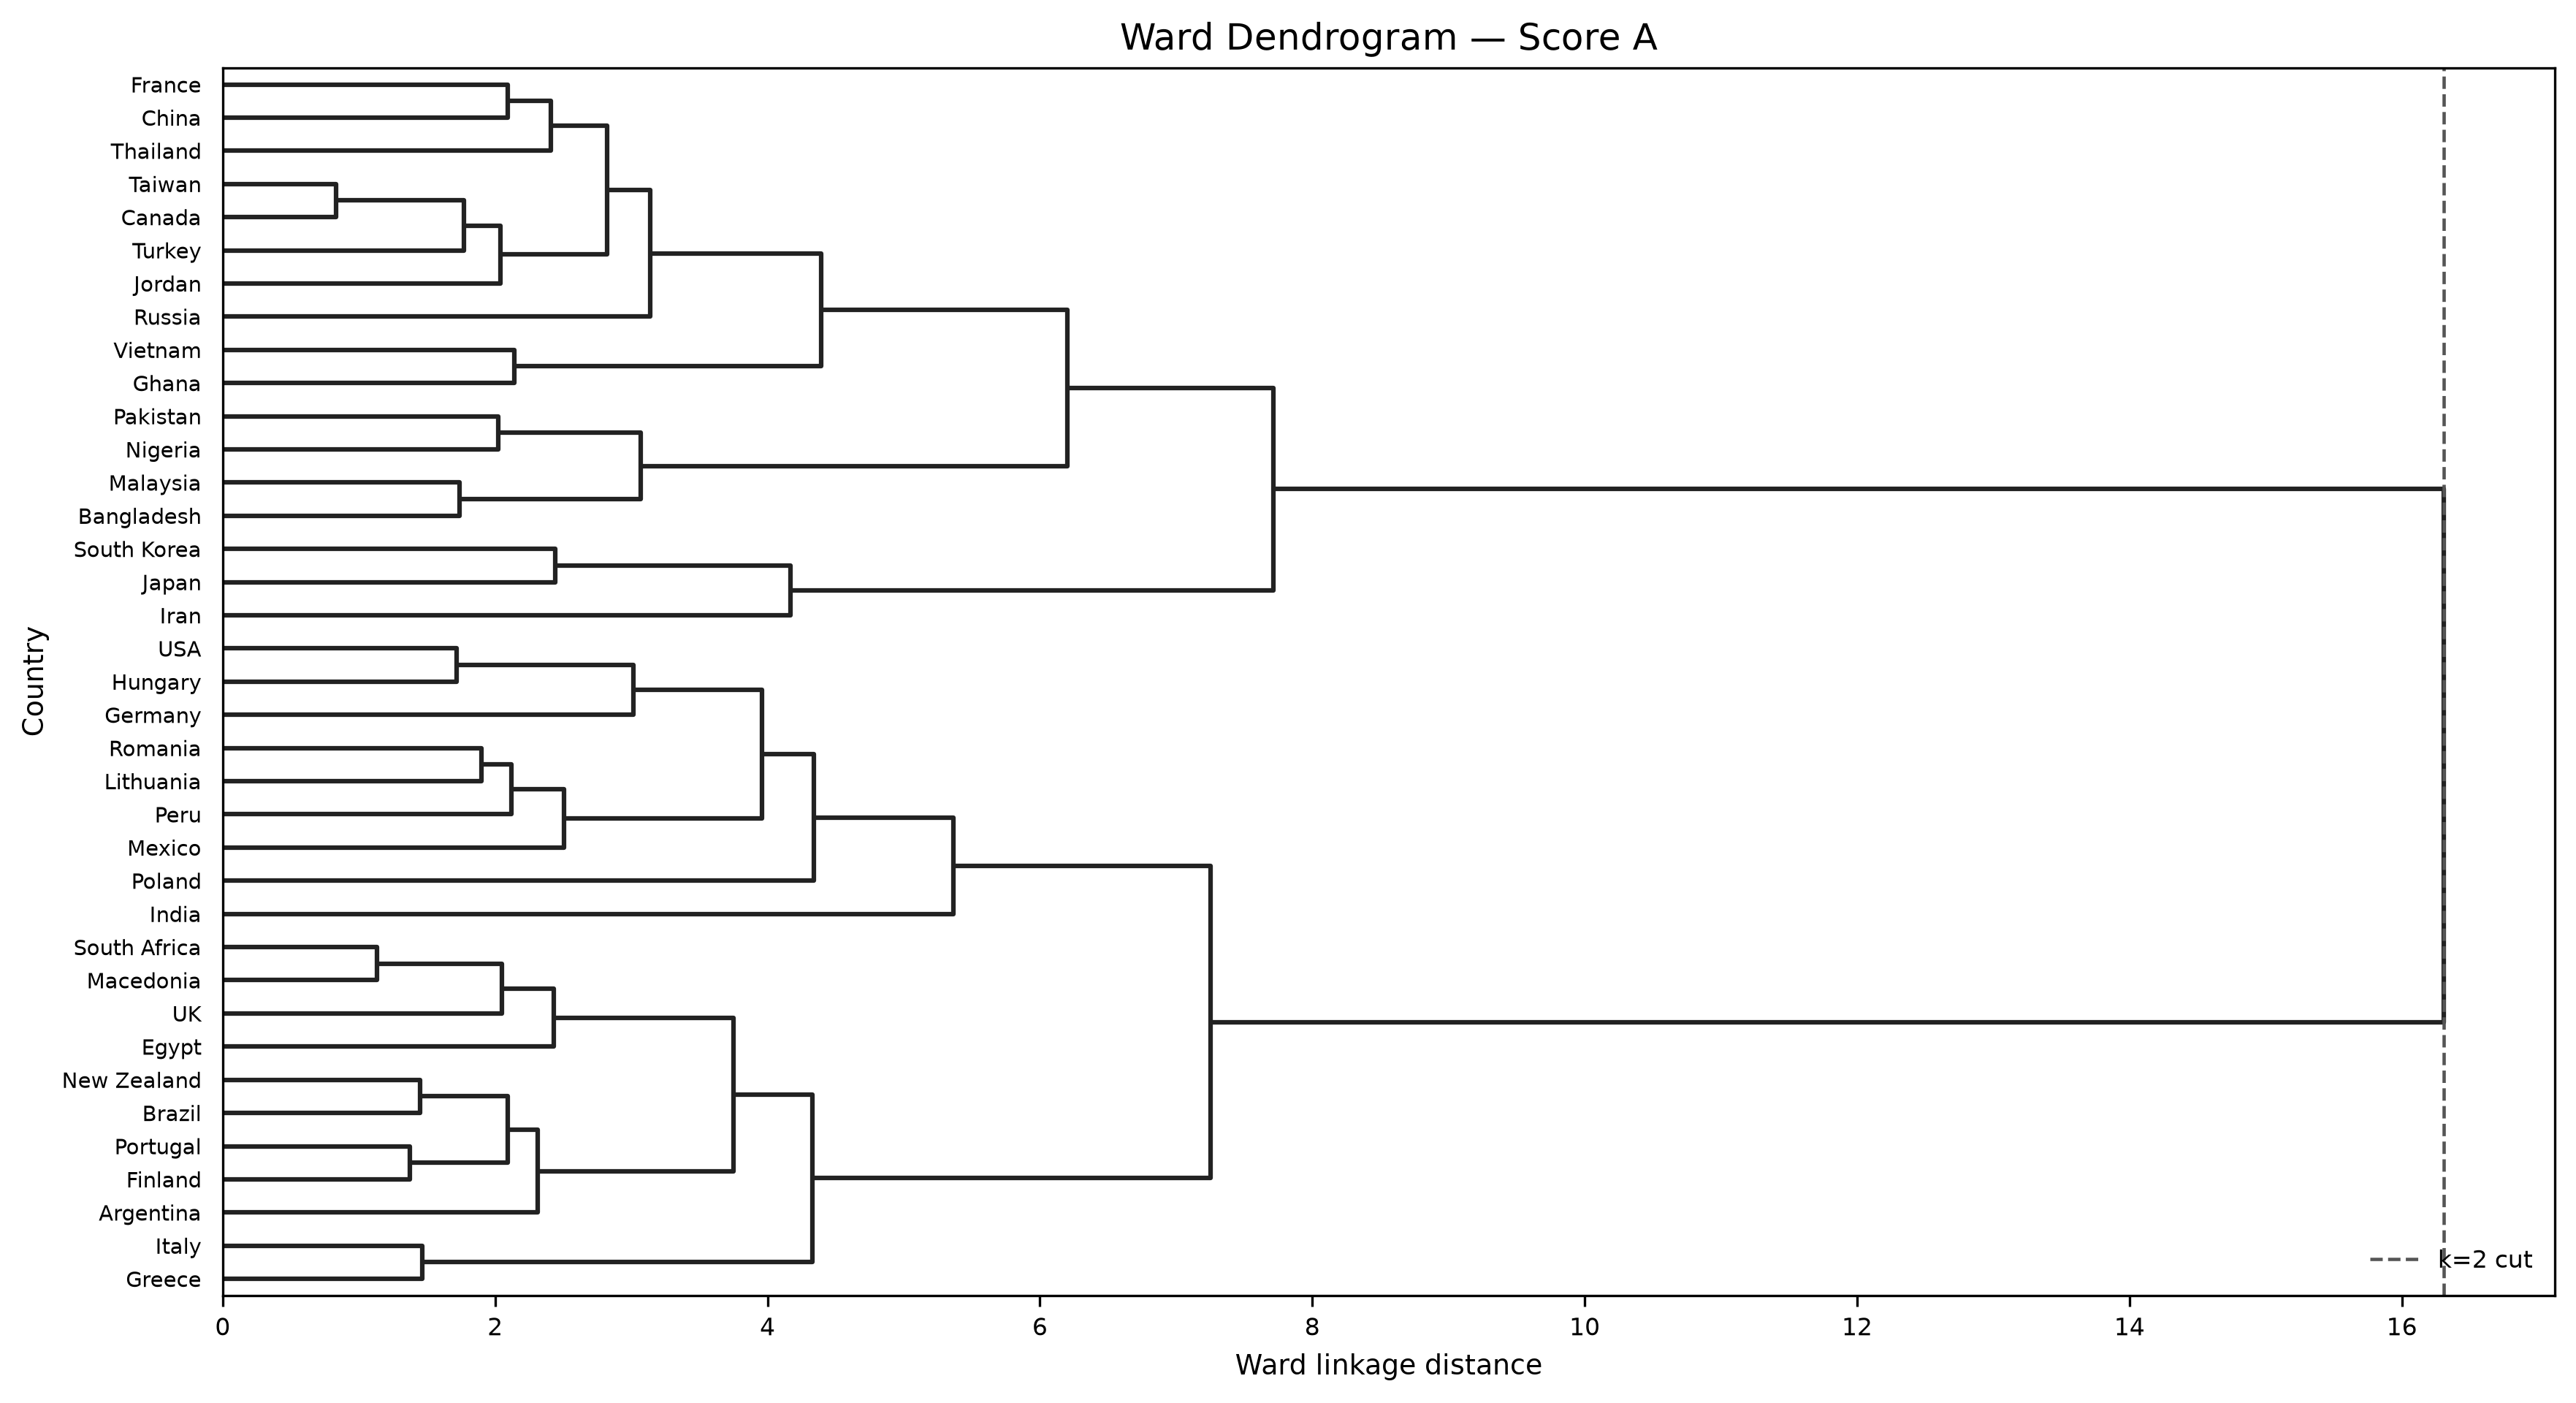
\includegraphics[width=0.96\textwidth]{dend_A.png}
\caption{Ward hierarchical dendrogram for standardized Score A. The dashed vertical line marks the two-cluster cut.}
\label{fig:dend_a}
\end{figure*}

\begin{figure*}[!t]
\centering
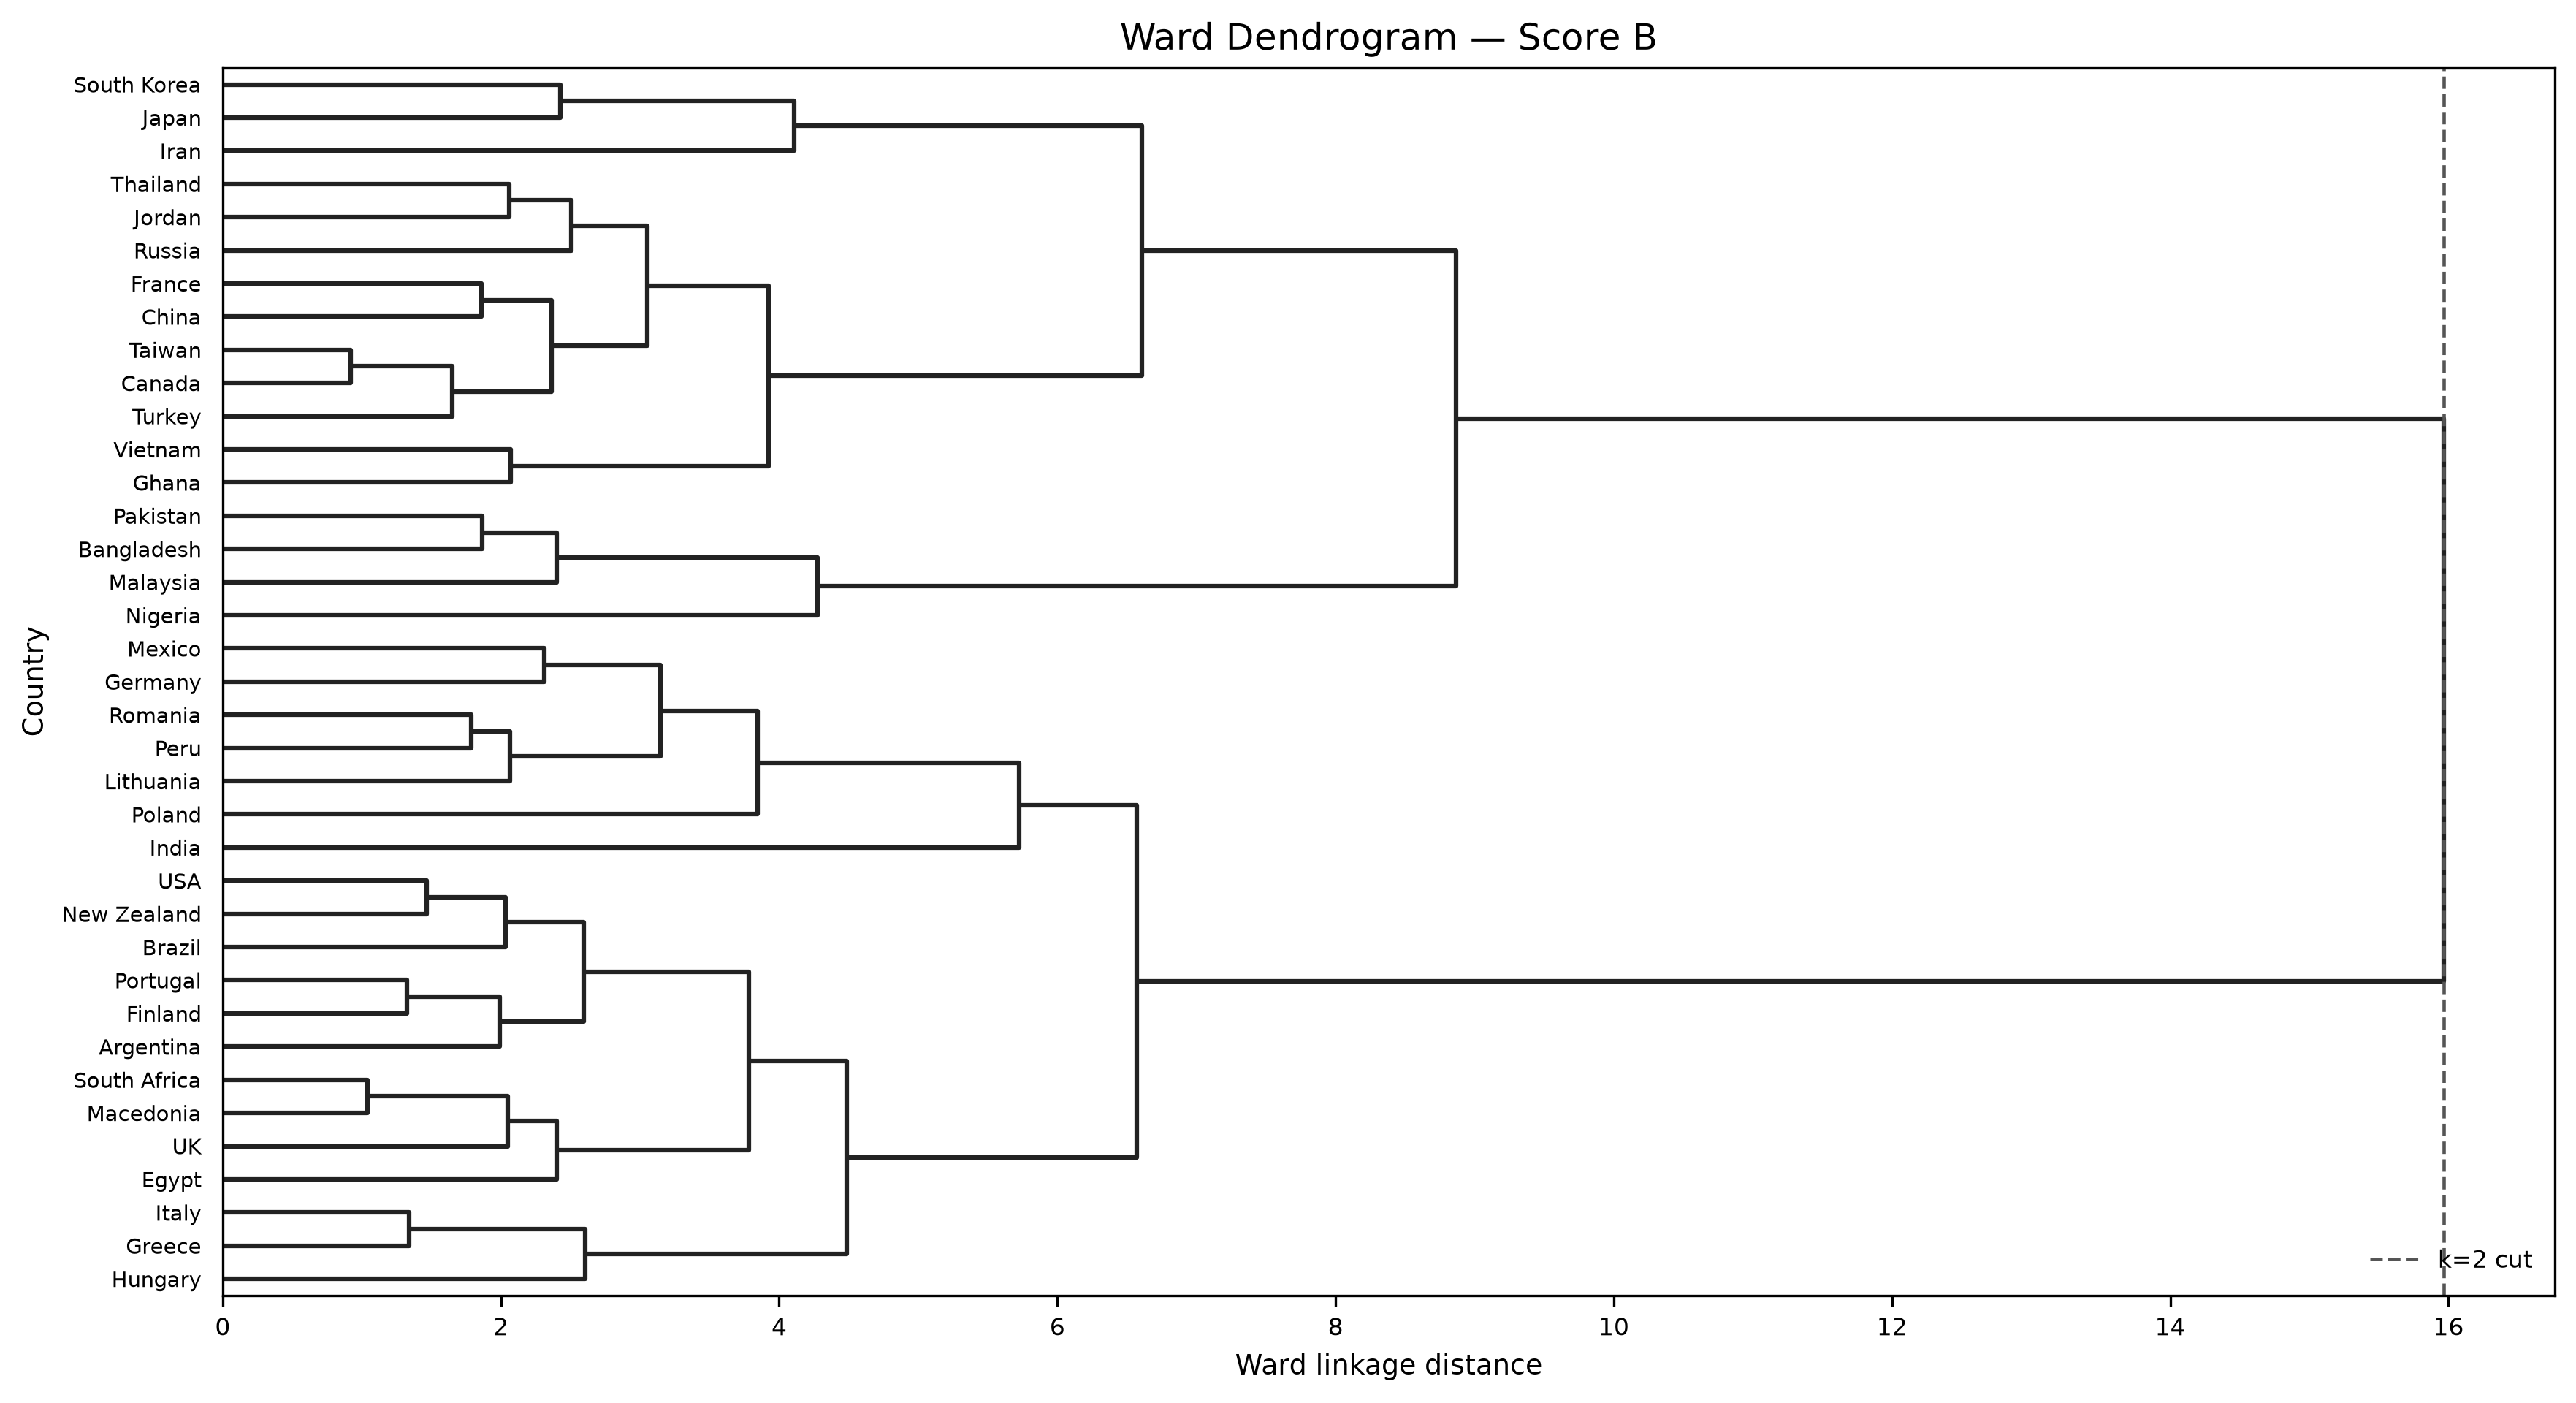
\includegraphics[width=0.96\textwidth]{dend_B.png}
\caption{Ward hierarchical dendrogram for standardized Score B. The dashed vertical line marks the two-cluster cut.}
\label{fig:dend_b}
\end{figure*}

\begin{figure*}[!t]
\centering
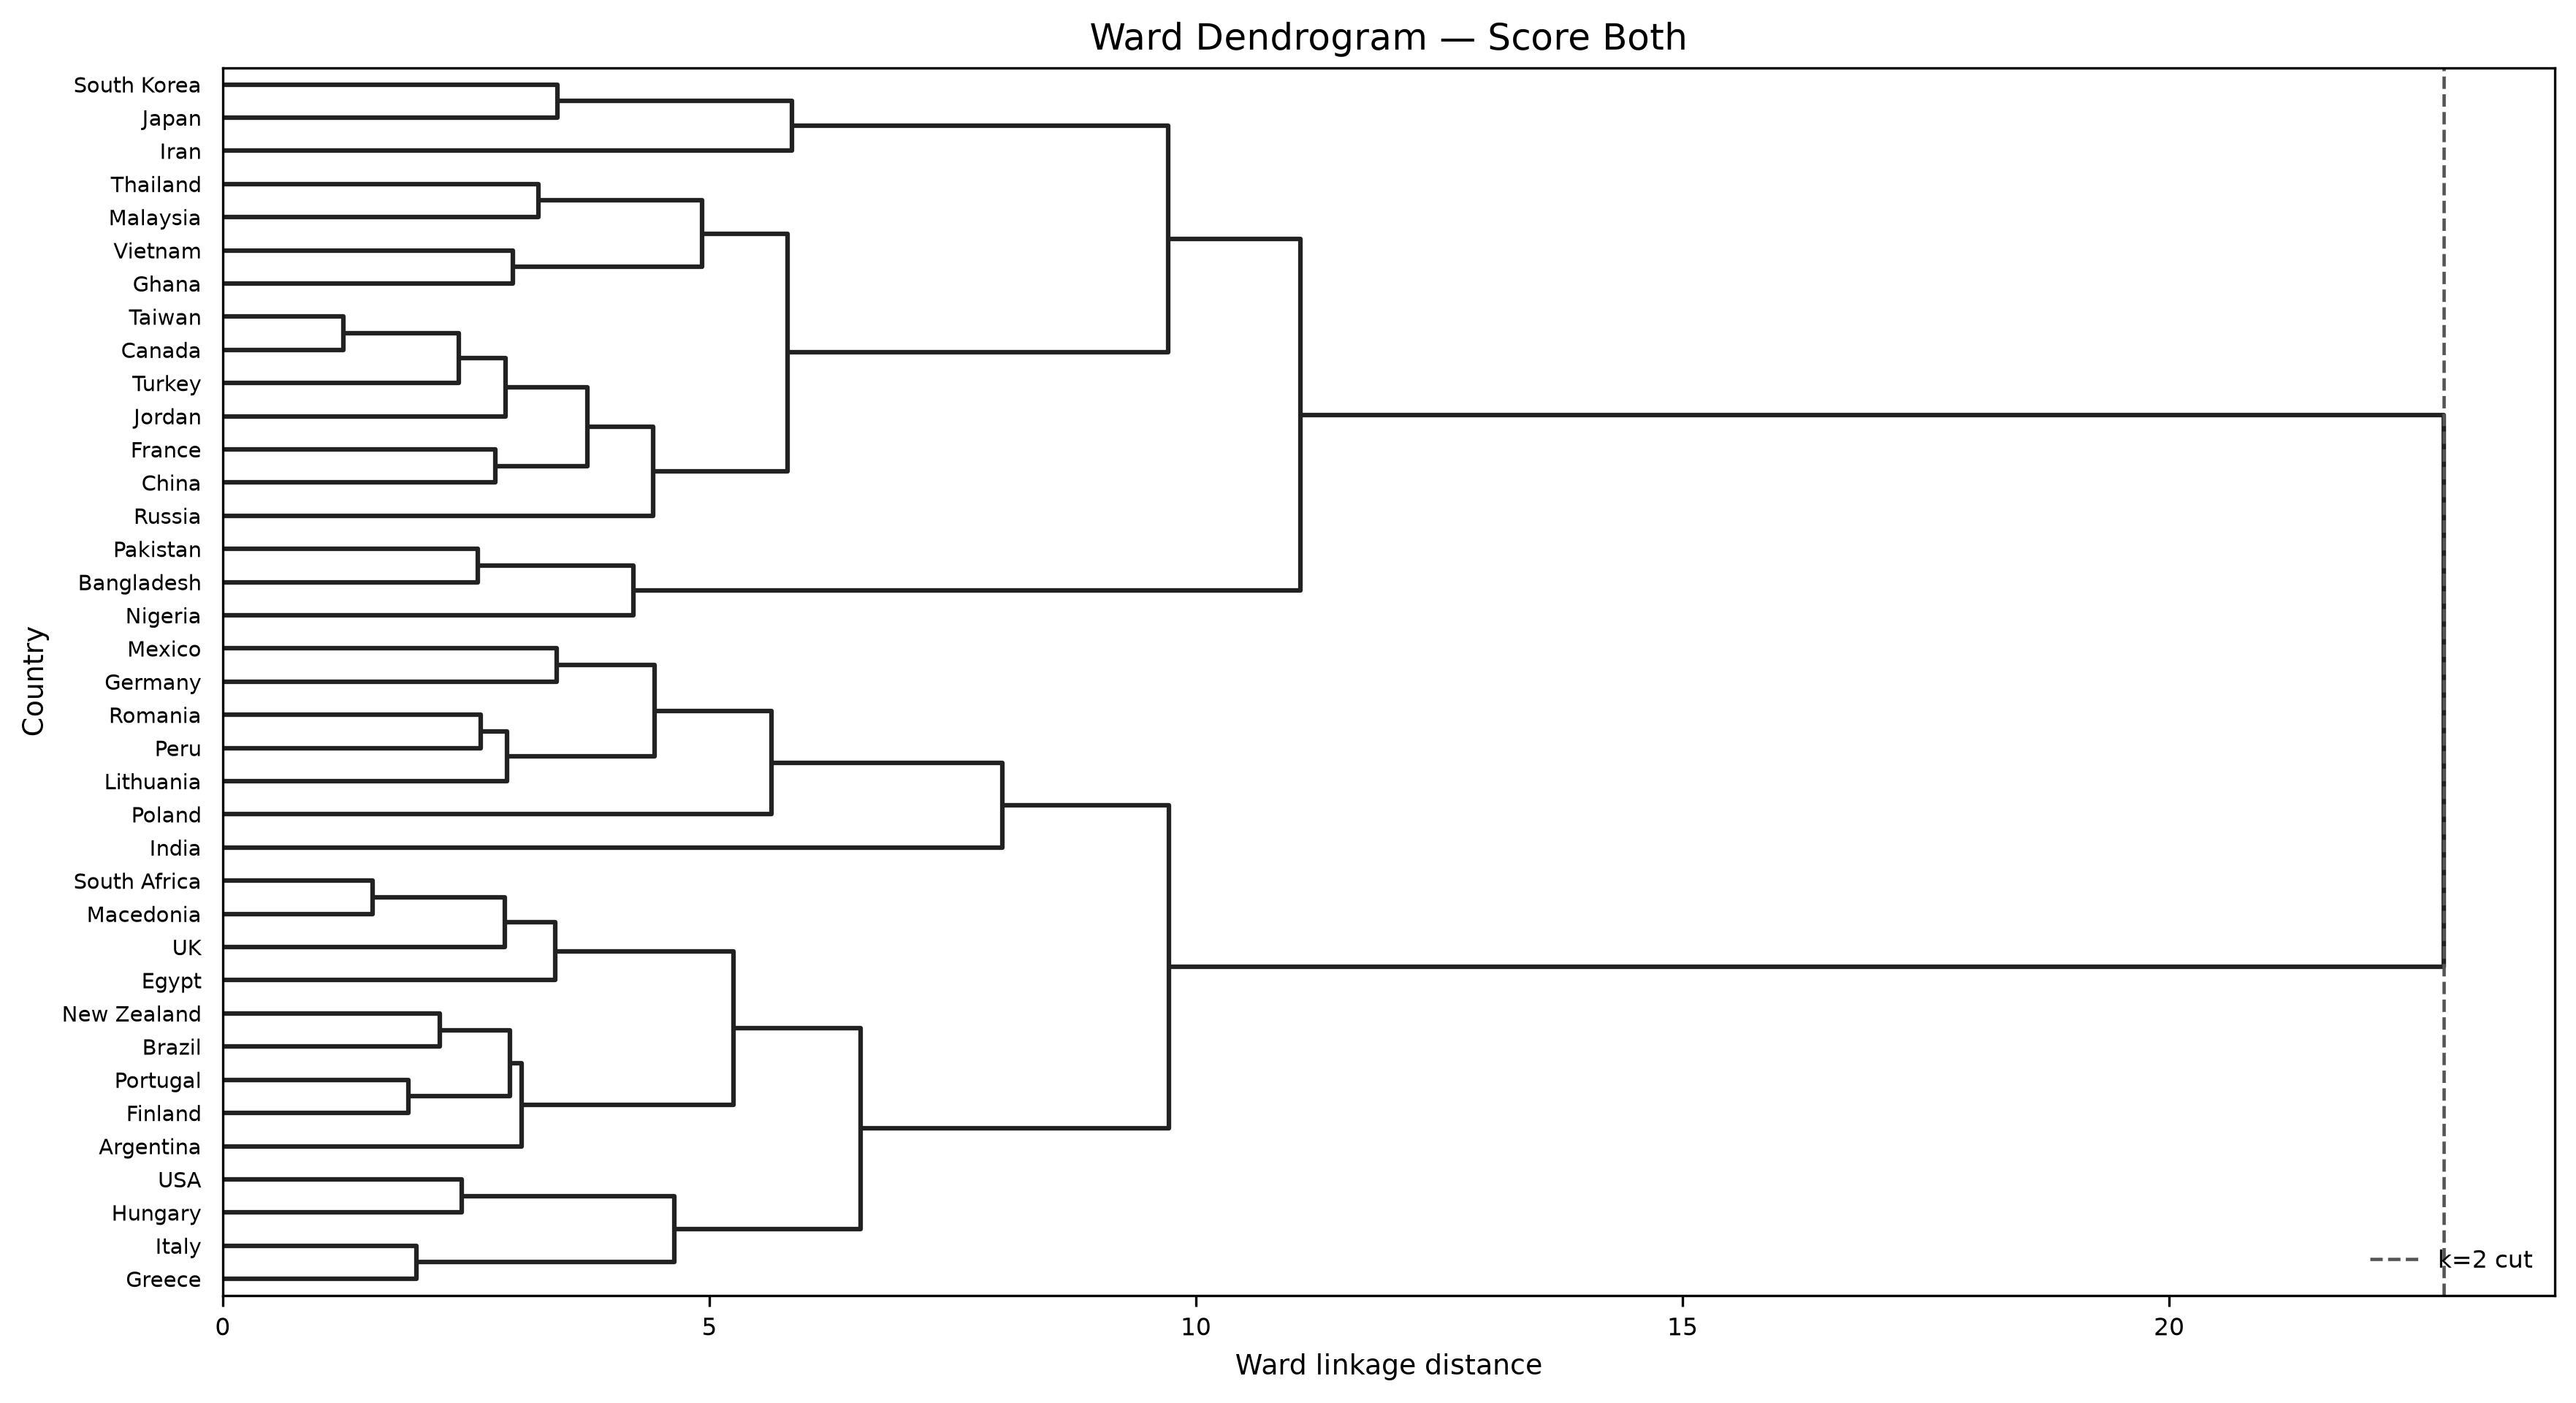
\includegraphics[width=0.96\textwidth]{dend_Both.png}
\caption{Ward hierarchical dendrogram for the standardized combined Score A and Score B features. The dashed vertical line marks the two-cluster cut.}
\label{fig:dend_both}
\end{figure*}

\begin{figure}[t]
\centering
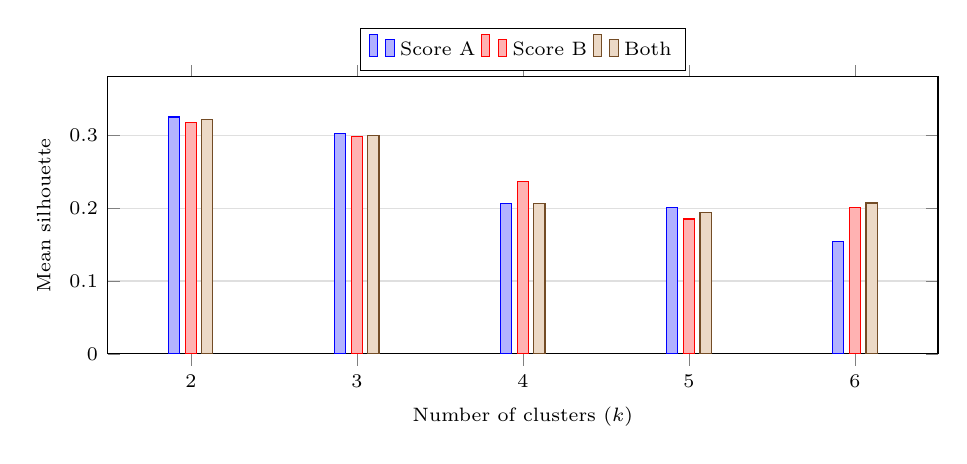
\begin{tikzpicture}
\begin{axis}[ybar,bar width=4pt,width=\columnwidth,height=5.1cm,
 xlabel={Number of clusters ($k$)},ylabel={Mean silhouette},
 xmin=1.5,xmax=6.5,ymin=0,ymax=0.38,xtick={2,3,4,5,6},
 legend style={font=\scriptsize,at={(0.5,1.02)},anchor=south,legend columns=3},
 tick label style={font=\scriptsize},label style={font=\scriptsize},
 ymajorgrids=true,grid style={gray!25}]
\addplot coordinates {(2,0.325)(3,0.302)(4,0.206)(5,0.201)(6,0.154)};
\addplot coordinates {(2,0.318)(3,0.298)(4,0.237)(5,0.185)(6,0.201)};
\addplot coordinates {(2,0.321)(3,0.299)(4,0.206)(5,0.194)(6,0.207)};
\legend{Score A,Score B,Both}
\end{axis}
\end{tikzpicture}
\caption{K-means silhouette scores across the evaluated cluster counts. The maximum is at $k=2$ for all three representations.}
\label{fig:silhouette}
\end{figure}

\Cref{fig:profile} visualizes the combined-solution group means on Score A. These are the supplied values' means, not directional evaluations: the scoring documentation does not tell us whether higher values indicate more or less of the named construct. The contrast is nevertheless useful for identifying which issue dimensions distinguish the groups.

\begin{figure}[t]
\centering
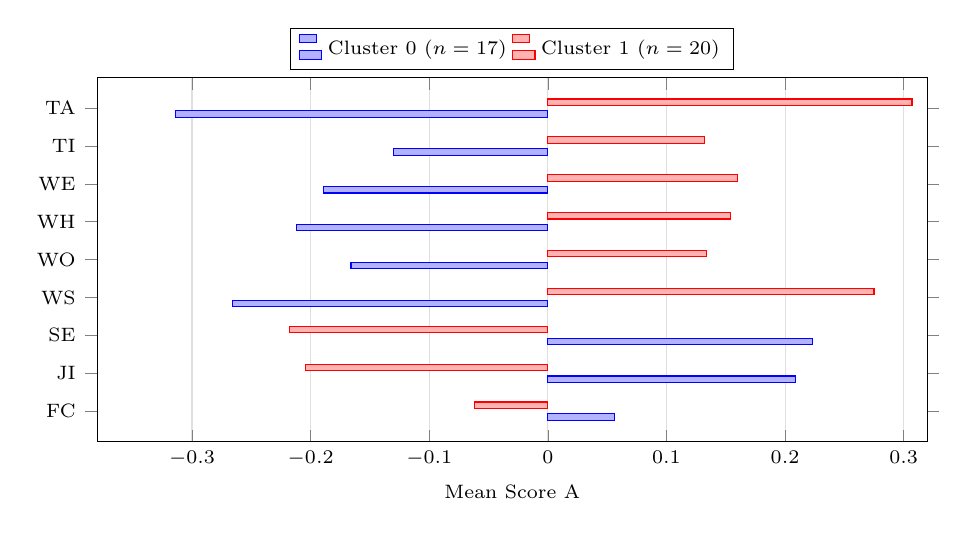
\begin{tikzpicture}
\begin{axis}[xbar,width=\columnwidth,height=6.2cm,
 xlabel={Mean Score A},xmin=-0.38,xmax=0.32,
 ytick={0,...,8},yticklabels={TA,TI,WE,WH,WO,WS,SE,JI,FC},
 y dir=reverse,legend style={font=\scriptsize,at={(0.5,1.02)},anchor=south,legend columns=2},
 tick label style={font=\scriptsize},label style={font=\scriptsize},
 xmajorgrids=true,grid style={gray!25},bar width=2.3pt]
\addplot coordinates {(-0.314,0)(-0.130,1)(-0.189,2)(-0.212,3)(-0.166,4)(-0.266,5)(0.223,6)(0.209,7)(0.056,8)};
\addplot coordinates {(0.307,0)(0.132,1)(0.160,2)(0.154,3)(0.134,4)(0.275,5)(-0.218,6)(-0.204,7)(-0.062,8)};
\legend{Cluster 0 ($n=17$),Cluster 1 ($n=20$)}
\end{axis}
\end{tikzpicture}
\caption{Combined k-means cluster means by issue for Score A. Abbreviations follow the definitions in the Introduction.}
\label{fig:profile}
\end{figure}

\section{Hypotheses / Theory Building}
We set three expectations. First, highly correlated score pairs should recover similar country groups. Second, a shared work-experience pattern should separate countries on several issues, not one. Third, regional and development context may account for some membership differences; that claim requires country covariates, not labels alone.

The first expectation holds at $k=2$: Score A, Score B, and the combined set produce identical k-means memberships. Cluster means differ on all nine Score A issues. For a limited macroeconomic check, we cross-tabulated the selected groups against the World Bank's FY2027 income classification, which uses 2025 GNI per capita~\cite{wb}. This is a current descriptive comparison; the workbook does not report when the worker scores were collected, so the years may not match. The classification is not a model input and does not explain the split. Comparable international ICT-skill data remain sparse: ITU reports that 40 countries provided comparable data in its 2024 collection~\cite{itu}.

\section{Analysis}
\subsection{Choice of $k$ and method}
For the combined set, mean silhouette is 0.321 at $k=2$, 0.299 at $k=3$, and 0.206 at $k=4$. Score A and B also peak at $k=2$ (0.325 and 0.318). Inertia falls from 405.6 at $k=2$ to 347.0 at $k=3$ and 299.0 at $k=4$, then declines through $k=8$. No sharp elbow appears. The Ward trees show the same two-cluster cut for each feature set. Silhouette, parsimony, and agreement favor $k=2$ for this sample. The $k=3$ and $k=4$ solutions divide it further but are less consistent across score sets.

At $k=2$, Ward and k-means agree for A, B, and the combined set (ARI=1.000 each). The three k-means partitions also agree (ARI=1.000). Agreement weakens at higher $k$: Score A versus B gives ARI=0.708 at $k=3$ and 0.428 at $k=4$. Average linkage on the combined matrix gives ARI=0.010 against k-means. The two-group result depends on the linkage rule.

\subsection{Country groups and profiles}
The combined k-means solution assigns 17 countries to Cluster 0 and 20 to Cluster 1 (\Cref{tab:membership}). The labels are arbitrary. USA (0.492), New Zealand (0.487), Peru (0.443), Lithuania (0.440), and Portugal (0.439) have the largest silhouettes. Russia is the only country below 0.10, at $-0.010$. Egypt (0.144), Canada (0.151), and Ghana (0.184) also lie near the boundary. These values rank assignment separation, not country outcomes.

\begin{table*}[t]
\centering
\caption{Country membership in the selected combined k-means solution ($k=2$).}
\label{tab:membership}
\small
\begin{tabular}{p{0.08\textwidth}p{0.84\textwidth}}
\toprule
Group & Countries \\
\midrule
Cluster 0 ($n=17$) & Bangladesh; Canada; China; France; Ghana; Iran; Japan; Jordan; Malaysia; Nigeria; Pakistan; Russia; South Korea; Taiwan; Thailand; Turkey; Vietnam \\
Cluster 1 ($n=20$) & Argentina; Brazil; Egypt; Finland; Germany; Greece; Hungary; India; Italy; Lithuania; Macedonia; Mexico; New Zealand; Peru; Poland; Portugal; Romania; South Africa; UK; USA \\
\bottomrule
\end{tabular}
\end{table*}

The largest Score B mean gaps occur on work satisfaction (12.596 versus 14.143), work exhaustion (11.987 versus 13.412), turnaway intention (10.294 versus 12.026), self-efficacy (8.769 versus 7.574), and job insecurity (6.838 versus 5.828). Score A has the same group ordering on these issues. We cannot call either group more satisfied or more insecure; score direction is absent from the documentation.

The income cross-tab gives a second, qualified view of the split. Cluster 0 contains 6 high-, 7 upper-middle-, and 4 lower-middle-income economies; Cluster 1 contains 12, 6, and 2, respectively. No sampled economy is currently classified as low-income. Thus Cluster 1 has a larger high-income share (60\% versus 35\%), while both groups span income categories. The two sets are not simply a rich-country and developing-country division.

\begin{table}[t]
\centering
\caption{Current World Bank income group by selected cluster; counts and within-cluster shares.}
\label{tab:income}
\small
\begin{tabular}{lrrr}
\toprule
Income group & Cluster 0 & Cluster 1 & Total \\
\midrule
High & 6 (35\%) & 12 (60\%) & 18 \\
Upper-middle & 7 (41\%) & 6 (30\%) & 13 \\
Lower-middle & 4 (24\%) & 2 (10\%) & 6 \\
Low & 0 (0\%) & 0 (0\%) & 0 \\
\bottomrule
\end{tabular}
\end{table}

Membership also follows region in several parts of the sample. Cluster 0 contains all four East Asian, all three Southeast Asian, and all three Middle Eastern cases as coded here. Cluster 1 contains all four Latin American and six of seven Western European cases. South Asia and Africa split across clusters; North America divides evenly. Canada and France fall in Cluster 0, India in Cluster 1. Regional labor markets, education systems, and technology policy could shape ICT work, but none is measured here. Connectivity can affect workers' access to training and employment; ICT skills and access are therefore plausible follow-up variables, not explanations established by these clusters~\cite{wbaccess,itu}.

\subsection{Assumptions and limits}
The distance model assumes comparable measurements across countries and no score-direction reversals. The supplied files cannot verify either assumption. Correlated issues also let overlapping constructs influence the 18-feature distance more than once. PCA records this concentration; it does not remove it. We retained the flagged extremes.

In 37 leave-one-country-out refits, every reduced-sample partition has ARI=1.000 against the corresponding subset of the full-sample partition. The selected split is stable to deletion of any one country under this scaling and method. This does not establish stability to new samples, changes in score construction, or alternative scaling. The low silhouette for Russia still marks an ambiguous individual assignment; stable memberships do not make every country's fit strong.

\section{Recommendations}
\begin{enumerate}
\item \textbf{Obtain the score specification.} Ask the data owner for construction, range, direction, and evidence of cross-country comparability. Until then, label groups by issue profile; do not call a score high or low in welfare terms.
\item \textbf{Review boundary cases first.} Russia has silhouette $-0.010$; Egypt, Canada, and Ghana score 0.144, 0.151, and 0.184. The partition survives single-country deletion, including these cases, but Russia remains closest to the decision boundary.
\item \textbf{Join contemporaneous country measures to worker profiles.} Add GNI per capita, ICT employment and vacancies, labor-market protections, broadband access and cost, tertiary or STEM education, and digital policy measures. The current income cross-tab is only a time-mismatched description; connectivity and skills are relevant because they condition access to digital work and training, but their association with this partition has not been tested~\cite{wbaccess}.
\item \textbf{Validate before targeting policy.} Test the split on a new worker sample and compare memberships across k-means, Ward, and average linkage. The current method comparison shows that linkage choice changes the result.
\end{enumerate}

\begin{thebibliography}{9}
\bibitem{task} DOM207--DOM3007--DOM6401, ``MP3: Cluster 37 Countries on 9 ICT-Worker Issues,'' project brief, supplied course task PDF, 2026.
\bibitem{definitions} International Monetary Fund, ``General Description of ICT Workers' Individual Issues,'' supplied dataset documentation PDF.
\bibitem{wb} World Bank, ``World Bank Country and Lending Groups,'' income-group methodology and current classifications. [Online]. Available: \url{https://datahelpdesk.worldbank.org/knowledgebase/articles/906519-world-bank-country-and-lending-groups}. Accessed: Nov. 2, 2026.
\bibitem{itu} International Telecommunication Union, ``Facts and Figures 2024: ICT skills,'' 2024. [Online]. Available: \url{https://www.itu.int/itu-d/reports/statistics/2024/11/10/ff24-ict-skills/}.
\bibitem{wbaccess} World Bank Group, ``Access,'' Digital and AI. [Online]. Available: \url{https://www.worldbank.org/ext/en/topic/digital-and-ai/access}. Accessed: Nov. 2, 2026.
\end{thebibliography}
\end{document}
